\chapter{Технологическая часть}

В данном разделе представлены выбор средств реализации, формат входных и выходных данных, требования к ПО, разработанные типы и структуры данных и алгоритмы, интерфейс ПО и тестирование ПО.

\section{Выбор средств реализации}
Для разработки программы был выбран язык C++.  Данный выбор обусловлен следующими факторами.

\begin{enumerate}[label=\arabic*)]
	\item C++ обладает высокой вычислительной производительностью, что очень важно для выполнения поставленной задачи \cite{cplusplusperfomance}.
	\item C++ поддерживает парадигму объектно-ориентированного программирования \cite{isocplusplus}.
	\item Для С++ существует большое количество научной и учебной литературы по алгоритмам компьютерной графики ($\approx17000$ результатов запроса <<c++ computer graphics algorithms>>в поисковой системе Академия Google).
\end{enumerate}

\section{Формат входных и выходных данных и обоснование выбора}

Входными данными для разрабатываемого программного обеспечения является информация о сцене (о всех её объетов). Для представления входных данных был выбран текстовый файл формата OBJ, так как согласно \cite{3d} формат OBJ:
\begin{enumerate}[label=\arabic*)]
	\item не привязан к какой-либо программе, работающей с 3D моделированием;
	\item занимает третье место в рейтинге по количеству моделей (на 17.10.2022 первое место в рейтинге, указанным в статье);
	\item является читаемым и редактируемым форматом, в отличие от бинарных форматов, таких как 3DS и MAX, которые занимают первое и второе места соответственно в рейтинге по количеству моделей.
\end{enumerate}

Выходными данными является растровое изображение. Из всех возможных форматов выходных данных (BMP, GIF, JPG, JPEG, PNG, PBM, PGM, PPM, XBM, XPM), которая предоставляет библиотека Qt, был выбран формат PNG, так как:
\begin{enumerate}[label=\arabic*)]
	\item формат PNG является графическим, что было необходимым для создания фильма с помощью утилиты ffmpeg \cite{ffmpeg};
	\item формат PNG является платформонезависимым, в отличие от формата BMP;
	\item согласно \cite{jpgvspng}, изображения в формате PNG более качественные, чем изображения в формате JPG по метрике типа PSNR (peak signal-to-noise ratio, пиковое отношение сигнала к шуму).
\end{enumerate}

\clearpage
\section{Требования к ПО}

На рисунке \ref{img:idef} представлена IDEF0-диаграмма ПО, характеризующая требования к ПО.
\begin{table}[H]
	\centering
	\begin{tabular}{p{1\linewidth}}
		\centering
		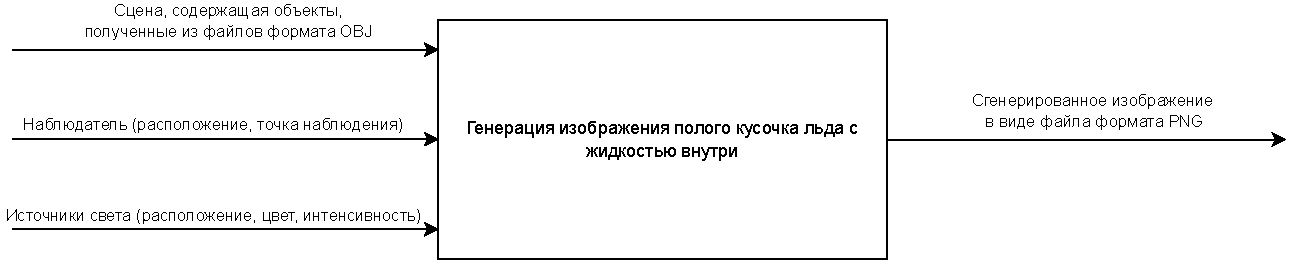
\includegraphics[width=1.0\linewidth]{include/idef0.pdf}
		\captionof{figure}{IDEF0-диаграмма ПО}
		\label{img:idef}
	\end{tabular}
\end{table}

\section{Реализация типов и структур данных}
Разработанные в конструкторской части \ref{types} типы и структуры данных были реализованы следующим образом.
\begin{enumerate}[label=\arabic*)]
	\item  Сцена представляет собой объект класса $Scene$ с приватными полями \lstinline[language={c++},keywordstyle=\color{black}]{_model} типа
	\lstinline[language={c++},keywordstyle=\color{black}]{std::vector<std::shared_ptr<Model>> } и \lstinline[language={c++},keywordstyle=\color{black}]{_light}  типа \lstinline[language={c++},keywordstyle=\color{black}]{std::vector<std::shared_ptr<Light>>} .
	\item  Модель представляет собой объекта класса $Model$ с приватными полями
	\lstinline[language={c++},keywordstyle=\color{blue}]{std::vector<QVector3D> _points} 
	, \lstinline[language={c++},keywordstyle=\color{black}]{std::vector<Triangle> _faces}  и \lstinline[language={c++},keywordstyle=\color{black}]{Material _material}.
	\item Материал представляет объекта класса $Material$ с приватными полями
	\lstinline[language={c++},keywordstyle=\color{blue}]{_ambient, _diffuse, _specular} , типа \lstinline[language={c++},keywordstyle=\color{black}]{QColor, _ka, _kd, _ks, _k_refl, _k_refr, _refraction_index} типа \lstinline[language={c++},keywordstyle=\color{black}]{double} и \lstinline[language={c++},keywordstyle=\color{black}]{_k} типа \lstinline[language={c++},keywordstyle=\color{black}]{int} 
	\item Камера представляет собой объект класса $Camera$ с приватными полями \lstinline[language={c++},keywordstyle=\color{black}]{_ic, _ij, _ik, _pos} типа \lstinline[language={c++},keywordstyle=\color{black}]{QVector3D} и \lstinline[language={c++},keywordstyle=\color{black}]{_img_width, _img_height} типа \lstinline[language={c++},keywordstyle=\color{black}]{int}.
	\item Источник света представляет собой объекта класса $Light$ с приватными полями \lstinline[language={c++},keywordstyle=\color{black}]{_position} типа \lstinline[language={c++},keywordstyle=\color{black}]{QVector3D}, \lstinline[language={c++},keywordstyle=\color{black}]{_color} типа \lstinline[language={c++},keywordstyle=\color{black}]{QColor} и \lstinline[language={c++},keywordstyle=\color{black}]{_intensity} типа \lstinline[language={c++},keywordstyle=\color{black}]{double}. 
\end{enumerate}

\section{Реализация алгоритмов}

В листингах \ref{raytracing1}  -- \ref{raytracing3} приведена реализация алгоритма испускания луча.

\begin{lstlisting}[label=raytracing1,caption=Реализация алгоритма испускания луча (начало), language=C++]
Color MainWindow::_cast_ray(Color& buf_color, const Ray ray, const int depth)
{
	Intersection intersect;
	
	Color color;
	
	if (_scene.intersect(ray, intersect) && depth <= N) {
		QVector3D reflect_dir = _reflects(-ray.get_dst(), intersect.norm);
		reflect_dir.normalize();
		QVector3D reflect_orig = QVector3D::dotProduct(reflect_dir, intersect.norm) < 0 ? intersect.point - intersect.norm * EPS : intersect.point + intersect.norm * EPS;
		Color reflect_color;
		if (intersect.material.get_k_refl() > 0)
			reflect_color = _cast_ray(buf_color, Ray(reflect_orig, reflect_dir), depth + 1);
		
		QVector3D refract_dir = _refract(ray.get_dst(), intersect.norm, intersect.material.get_refraction_index());
		refract_dir.normalize();
		QVector3D refract_orig = QVector3D::dotProduct(refract_dir, intersect.norm) < 0 ? intersect.point - intersect.norm * EPS : intersect.point + intersect.norm * EPS;
		Color refract_color;
		if (intersect.material.get_k_refr() > 0)
			refract_color = _cast_ray(buf_color, Ray(refract_orig, refract_dir), depth + 1);
		color.r = (intersect.material.get_ambient().r * intersect.material.get_ka());
		color.g = (intersect.material.get_ambient().g * intersect.material.get_ka());
		color.b = (intersect.material.get_ambient().b * intersect.material.get_ka());
\end{lstlisting}
\clearpage
\begin{lstlisting}[label=raytracing2,caption=Реализация алгоритма испускания луча (продолжение), language=C++]
		for (size_t k = 0; k < _scene.get_lights().size(); k++) {
			QVector3D L = _scene.get_lights()[k]->get_position() - intersect.point;
			L.normalize();
			
			double fator_dif = QVector3D::dotProduct(L, intersect.norm);
			double light_dist = (_scene.get_lights()[k]->get_position() - intersect.point).length();
			
			QVector3D shadow_orig = fator_dif <= EPS ? intersect.point - intersect.norm * EPS : intersect.point + intersect.norm * EPS;
			
			Intersection tmp_intersect;
			Ray tmp_ray = Ray(shadow_orig, L);
			
			if (_scene.intersect(tmp_ray, tmp_intersect) && (tmp_intersect.point - shadow_orig).length() < light_dist && fabs(tmp_intersect.material.get_k_refr()) < EPS) {
				continue;
			}
			
			if (fator_dif <= EPS)
				fator_dif = 0.0;
			
			color.r = color.r + _scene.get_lights()[k]->get_color().r * _scene.get_lights()[k]->get_intensity() * fator_dif * intersect.material.get_diffuse().r * intersect.material.get_kd();
			color.g = color.g + _scene.get_lights()[k]->get_color().g * _scene.get_lights()[k]->get_intensity() * fator_dif * intersect.material.get_diffuse().g * intersect.material.get_kd();
			color.b = color.b + _scene.get_lights()[k]->get_color().b * _scene.get_lights()[k]->get_intensity() * fator_dif * intersect.material.get_diffuse().b * intersect.material.get_kd();
\end{lstlisting}
\clearpage
\begin{lstlisting}[label=raytracing3,caption=Реализация алгоритма испускания луча (окончание), language=C++]
			QVector3D reflexao = _reflects(L, intersect.norm);
			double fator_esp = QVector3D::dotProduct(ray.get_vector(), reflexao);
			if (fator_esp <= EPS)
				fator_esp = 0.0;
			
			color.r = color.r + _scene.get_lights()[k]->get_color().r * _scene.get_lights()[k]->get_intensity() * pow(fator_esp, intersect.material.get_k()) * intersect.material.get_specular().r * intersect.material.get_ks();
			color.g = color.g + _scene.get_lights()[k]->get_color().g * _scene.get_lights()[k]->get_intensity() * pow(fator_esp, intersect.material.get_k()) * intersect.material.get_specular().g * intersect.material.get_ks();
			color.b = color.b + _scene.get_lights()[k]->get_color().b * _scene.get_lights()[k]->get_intensity() * pow(fator_esp, intersect.material.get_k()) * intersect.material.get_specular().b * intersect.material.get_ks();
			
			color.r = color.r + reflect_color.r * intersect.material.get_k_refl();
			color.g = color.g + reflect_color.g * intersect.material.get_k_refl();
			color.b = color.b + reflect_color.b * intersect.material.get_k_refl();
			
			color.r = color.r + refract_color.r * intersect.material.get_k_refr();
			color.g = color.g + refract_color.g * intersect.material.get_k_refr();
			color.b = color.b + refract_color.b * intersect.material.get_k_refr();
		}
		color.normalize();
	} else {
		color = Color(0.07, 0.07, 0.07);
	}
	buf_color = color;
	return color;
}
\end{lstlisting}

В листинге \ref{raytracing4}  приведена реализация алгоритма пересечения луча со сценой.

\begin{lstlisting}[label=raytracing4,caption=Реализация алгоритма пересечения луча со сценой, language=C++]
bool Scene::intersect(const Ray& ray, Intersection& intersect)
{
	double dist = std::numeric_limits<float>::max();
	;
	Intersection closest;
	
	for (auto iter = _objects.begin(); iter != _objects.end(); iter++) {
		
		Intersection inter = (*iter)->intersection(ray);
		
		if (inter.dist > 0.0 && inter.dist <= dist) {
			dist = inter.dist;
			closest = inter;
		}
	}
	
	if (fabs(dist - std::numeric_limits<float>::max()) < EPS)
	return false;
	
	intersect = closest;
	
	return true;
}
\end{lstlisting}

В листингах \ref{raytracing5} -- \ref{raytracing6}   приведена реализация алгоритма пересечения луча с объектом.

\begin{lstlisting}[label=raytracing5,caption=Реализация алгоритма пересечения луча с объектом (начало), language=C++]
Intersection Model::intersection(const Ray& ray) const
{
	Intersection intersectPoint;
	intersectPoint.dist = 0.0;
	
	if (!this->_ray_box_intersect(ray))
		return intersectPoint;
	
	float faceDist = std::numeric_limits<float>::max();
\end{lstlisting}
\begin{lstlisting}[label=raytracing6,caption=Реализация алгоритма пересечения луча с объектом (окончание), language=C++]
	float currDist;
	Triangle face;
	
	std::vector<Triangle>::const_iterator face_it;
	
	for (auto it = _faces.begin(); it != _faces.end(); ++it) {
		if (this->_ray_face_intersect(ray, *it, currDist) && fabs(currDist) < faceDist) {
			faceDist = currDist;
			face = *it;
			face_it = it;
		}
	}
	
	if (faceDist == std::numeric_limits<float>::max())
		return intersectPoint;
	
	intersectPoint.norm = this->get_normal(face, ray);
	intersectPoint.dist = faceDist;
	intersectPoint.point = ray.get_src() + ray.get_dst() * faceDist;
	intersectPoint.material = this->get_material();
	
	return intersectPoint;
}
\end{lstlisting}

В листингах \ref{raytracing9} -- \ref{raytracing10}   приведена реализация алгоритма пересечения луча с полигоном.
\begin{lstlisting}[label=raytracing9,caption=Реализация алгоритма пересечения луча с полигоном (начало), language=C++]
bool Model::_ray_face_intersect(const Ray& ray, const Triangle& face, float& ray_tvalue) const
{
	QVector3D edge1 = get_point(face.verts[1]) - get_point(face.verts[0]);
	QVector3D edge2 = get_point(face.verts[2]) - get_point(face.verts[0]);
	
	QVector3D pvec = QVector3D::crossProduct(ray.get_dst(), edge2);
	float det = QVector3D::dotProduct(edge1, pvec);
\end{lstlisting}
\clearpage
\begin{lstlisting}[label=raytracing10,caption=Реализация алгоритма пересечения луча с полигоном (окончание), language=C++]
	if (fabs(det) < EPS)
		return false;
	
	auto inv_det = 1. / det;
	
	QVector3D tvec = ray.get_src() - get_point(face.verts[0]);
	
	float bary_u = QVector3D::dotProduct(tvec, pvec) * inv_det;
	if (bary_u < 0.0 || bary_u > 1.0)
		return false;
	
	QVector3D qvec = QVector3D::crossProduct(tvec, edge1);
	float bary_v = QVector3D::dotProduct(ray.get_dst(), qvec) * inv_det;
	
	if (bary_v < 0.0 || bary_u + bary_v > 1.0)
		return false;
	
	ray_tvalue = static_cast<float>(QVector3D::dotProduct(edge2, qvec) * inv_det);
	
	return ray_tvalue > EPS;
}
\end{lstlisting}

\section{Описание интерфейса программы}

На рисунках \ref{img:gui1} -- \ref{img:gui3} представлен интерфейс программного продукта. На рисунке \ref{img:gui1} изображён режим работы с геометрией объектов, взаимодействуя с которым можно добавить объект на сцену, удалить объект со сцены, переместить, масштабировать и повернуть выбранный из выпадающего списка объект.  На рисунке \ref{img:gui2} представлен режим работы с источниками света. С помощью данного интерфейса можно добавить источник света на сцену, удалить источник света со сцены, изменить его свойства (расположение, интенсивность). На рисунке \ref{img:gui3} проиллюстрирован режим работы со свойствами материалов объектов, с помощью которого можно устанавливать параметры фонового освещения, диффузного освещения, зеркального освещения, коэффициенты отражения, преломления материалов объектов.

\begin{table}[H]
	\centering
	\begin{tabular}{p{1\linewidth}}
		\centering
		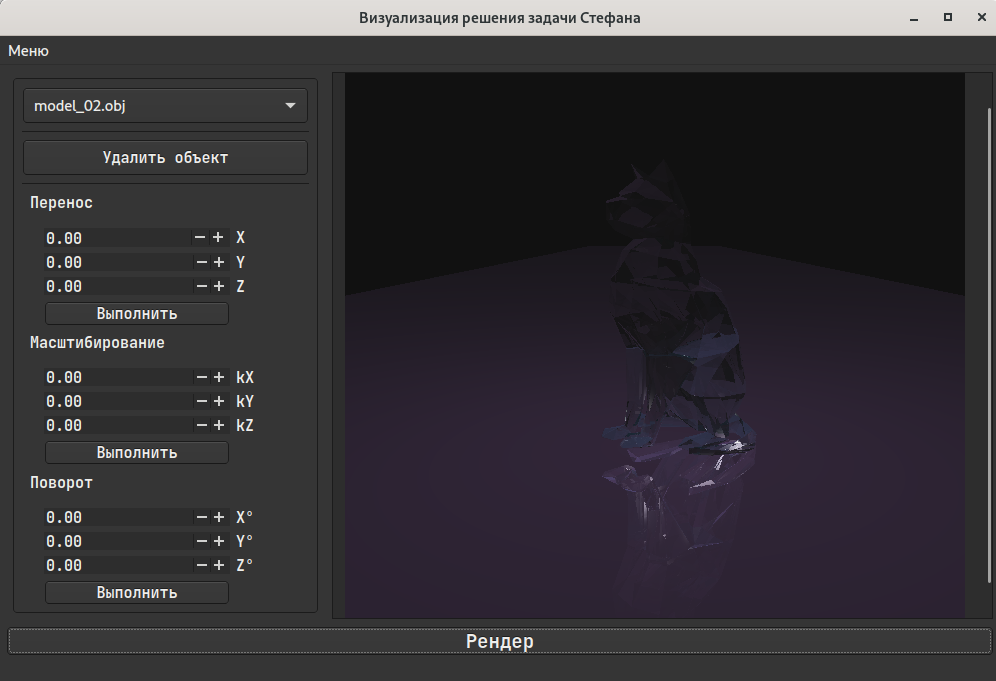
\includegraphics[width=0.85\linewidth]{include/gui1.png}
		\captionof{figure}{Интерфейс ПО (режим работы с геометрией объектов)}
		\label{img:gui1}
	\end{tabular}
\end{table}

\begin{table}[H]
	\centering
	\begin{tabular}{p{1\linewidth}}
		\centering
		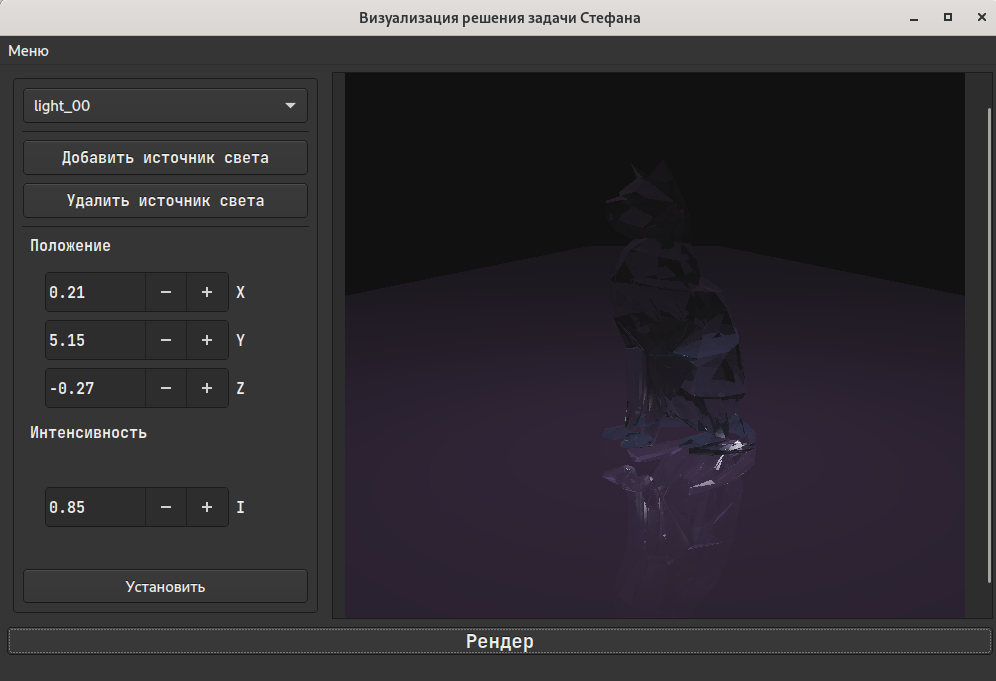
\includegraphics[width=0.85\linewidth]{include/gui2.png}
		\captionof{figure}{Интерфейс ПО (режим работы с источниками света)}
		\label{img:gui2}
	\end{tabular}
\end{table}

\begin{table}[H]
	\centering
	\begin{tabular}{p{1\linewidth}}
		\centering
		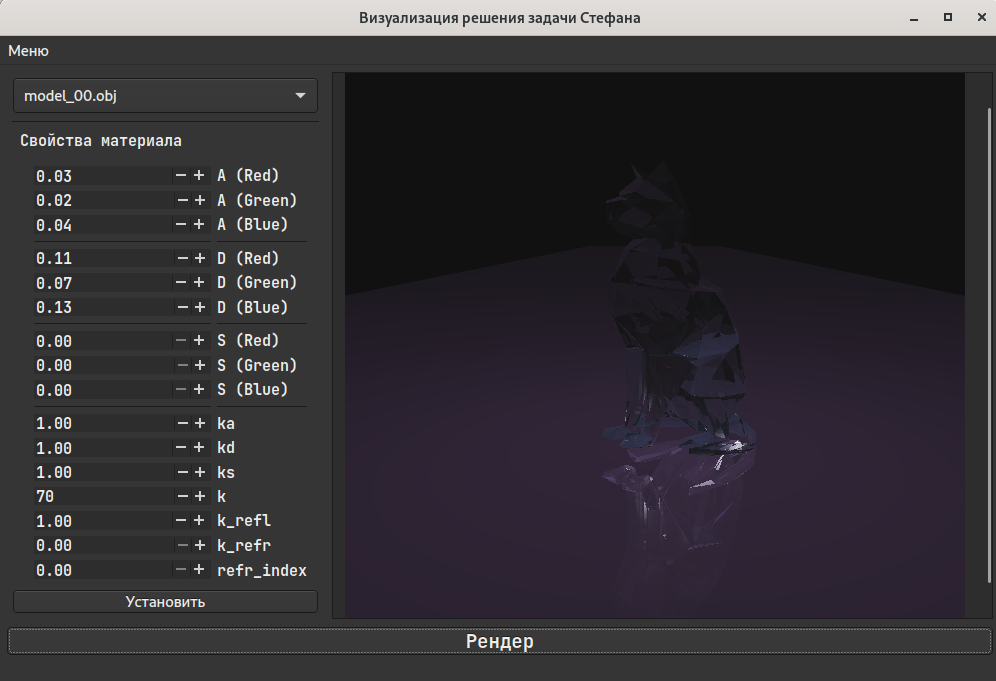
\includegraphics[width=0.85\linewidth]{include/gui3.png}
		\captionof{figure}{Интерфейс ПО (режим работы со свойствами материалов объектов)}
		\label{img:gui3}
	\end{tabular}
\end{table}

\section{Тестирование ПО}

Было проведено модульное тестирование всех неинтерфейсных модулей программы. Для тестирования был выбран фреймворк Qt Test \cite{qttest}. Результаты тестирования, обработанные утилитой lcov, представлены на рисунке \ref{img:lcov}.

\begin{table}[H]
	\centering
	\begin{tabular}{p{1\linewidth}}
		\centering
		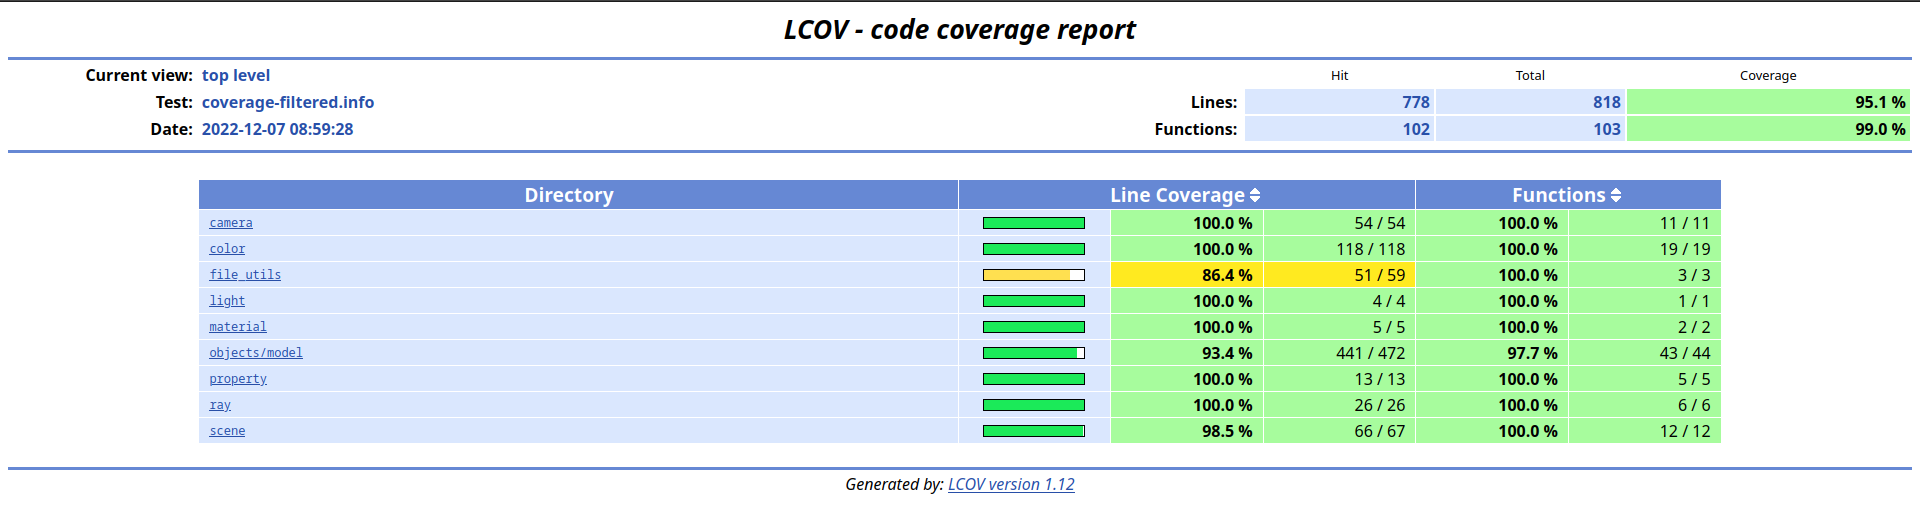
\includegraphics[width=1.0\linewidth]{include/lcov.png}
		\captionof{figure}{Результаты модульного тестирования}
		\label{img:lcov}
	\end{tabular}
\end{table}

\section{Выводы из технологической части}

В данном разделе были обоснованы выбор средств реализации, формат входных и выходных данных, разработаны типы и структуры данных и алгоритмы, рассмотрен интерфейс разработанного ПО и проведено тестирование разработанного продукта.
